\chapter{Namespace XML}

Cette partie décrit la représentation C++ d'un XML ainsi que les traitements associés.

Les hypothèse suivantes sont également formulées :
\begin{itemize}
    \item Les documents XML à parser ne contiendront pas de DTD interne
    \item Les Processing Instruction (PI) ne contiendront que des attributs
    \item Aucune référence ne sera présente dans les documents XML\\
\end{itemize}


\section{Diagramme de classes}
    Les classes ici décrites seront rattachées au \textit{\lstinline$namespace Xml$} défini en C++.

    \begin{landscape}
    \begin{figure}[h!]
        \centering
        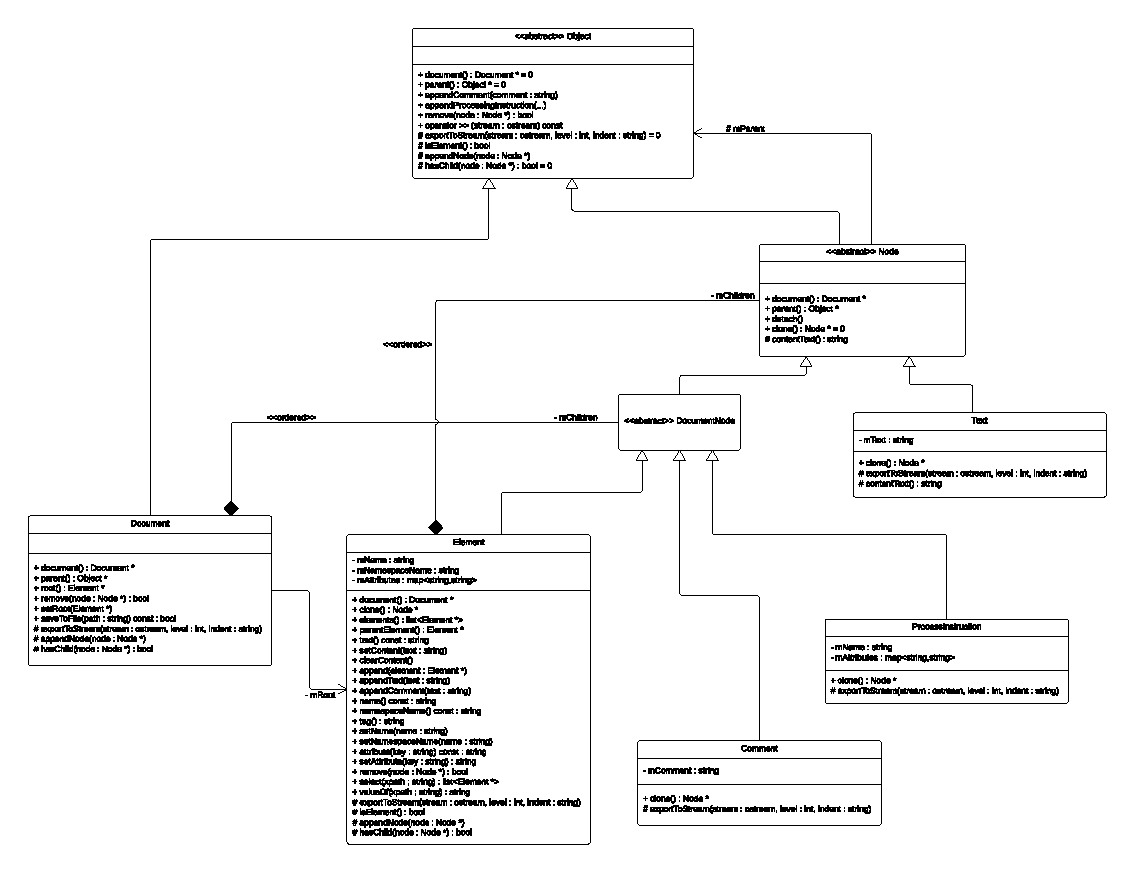
\includegraphics[width=0.9\linewidth]{images/xml-uml.pdf}
        \caption{Diagramme de classes de l'arborescence XML}
        \label{classDiagram}
    \end{figure}
    \end{landscape}


\section{Classes}
    \subsection{Log}
        La class \lstinline$Log$ a pour unique mission de stocker l'ensemble de l'output du parseur \textit{XML} telle que~:

        \begin{itemize}
            \item Erreurs lexicales~;
            \item Erreurs syntaxique~;
            \item Erreurs semantiques.
        \end{itemize}

    \subsection{Object}
        Pour optimiser et éviter au maximum la redondance de données dans notre arbre d'héritage de l'implementation \textit{XML}, nous nous sommes inspirés de la très célèbre librarie \textit{Qt} avec son \lstinline$QObject$. Ainsi nous avons notre \lstinline$Xml::Object$ offrant les avantages que vous trouverez dans les sous-sections suivantes.

    \subsection{Node}
    Ainsi, nous partons du principe qu'un document XML n'est en réalité qu'un arbre ayant des noeuds (\lstinline$Node$) étant des objects XML, mais de natures differents (commentaires, texte, élément \ldots). Certains de ces noeuds seront des feuilles de l'arbre (le noeud de commentaire par exemple).

        Ici se trouve déjà un avantage du \lstinline$Xml::Object$ car chaque \lstinline$Node$ connait son \lstinline$Object$ parent à l'aide de \lstinline$mParent$ pouvant être un \lstinline$Element$ ou un \lstinline$Document$. Ainsi, on peut à partir d'un noeud, retrouver le \lstinline$Document$ dans lequel il se trouve simplement en remontant l'arbre.

    \subsection{DocumentNode}
        Le \lstinline$DocumentNode$ est une spécialisation de \lstinline$Node$, mais ayant seulement une particularité' sémantique~: seul ses classes fillent peuvent avoir pour parent, un \lstinline$Element$ par hertiage de \lstinline$Node$, mais aussi un \lstinline$Document$ au contraire de la classe \lstinline$Text$ ne pouvant avoir pour parent qu'un \lstinline$Element$.

    \subsection{Document}
        Un \lstinline$Document$ est un \lstinline$Node$ composé de \lstinline$DocumentNode$. Parmis ces \lstinline$DocumentNode$, un seul et unique \lstinline$Element$ racine compose cette liste. Mais afin de pouvoir retrouver cette racine du document en complexité $O(1)$, \lstinline$DocumentNode$ dispose aussi d'un attributs \lstinline$mRoot$ dedié à cette tache.

        Cette même liste de \lstinline$DocumentNode$ est ordonnée afin de garentir l'ordre des noeuds au chargement et à l'exportation du document \textit{XML}. L'\lstinline$Element$ racine fait partie de cette liste afin d'éviter d'avoir à gerer deux listes de noeuds (ceux avant et ceux après).

    \subsection{Comment}
        \lstinline$Comment$ est un \lstinline$DocumentNode$ car il peut être n'importe où dans le document \textit{XML}~: dans un \lstinline$Element$ ou bien en dehors de l'élément racine du document.

    \subsection{ProcessingInstruction}
        Une \lstinline$ProcessingInstruction$ est aussi un \lstinline$DocumentNode$ d'après les spécifications officielles de \textit{XML}. Mais en accord avec l'hypothèse énoncée précédemment, une \lstinline$ProcessingInstruction$ ne contient qu'un nom et une map d'attributs.

    \subsection{Text}
        Un noeud de texte est naturellement décrit par une chaîne de caractères \lstinline$mText$. Celui-ci ne dérive pas de la classe \lstinline$DocumentNode$ puisque, si son contenu s'apparente à celui d'un noeud Comment, il ne peut en revanche être contenu par une instance de \lstinline$Element$. Il est donc nécessaire d'ajouter le niveau de spécialisation \lstinline$DocumentNode$ afin d'éviter une relation ne respectant pas les spécifications standards \textit{XML}.

    \subsection{Element}
        Un \lstinline$Element$ \textit{XML} est un \lstinline$DocumentNode$. Il possède une liste d'\lstinline$Element$ enfants \lstinline$mChildren$. Cette classe peut aussi représenter la racine d'un \lstinline$Document$.

        Celui ci est defini avec un nom de balise (\lstinline$mName$) mais aussi d'un espace de nom (\lstinline$mNamespaceName$). La concatenation de ces deux derniers forment le tag (namespace + ":" + nom) de l'\lstinline$Element$. Le nom du membre \lstinline$mNamespaceName$ au lieu de \lstinline$mNamespace$ a été effectué pour éviter la collision avec le mot clef du language C++ \lstinline$namespace$ avec son getter théorique \lstinline$Xml::Element::namespace()$ remplacer par \lstinline$Xml::Element::namespaceName()$.

        Un \lstinline$Element$ possède un ensemble non-ordonné d'attributs étant simplement une map ayant une association $clef \leftarrow valeur$. Par soucis de déterminisme, nous les exportons par ordre alphabétique des clefs.

        Enfin un \lstinline$Element$ possède une liste ordonnée de noeuds (\lstinline$Node$). Mais cette liste est inaccessible à l'utilisateur. En effet, nous ne voulons pas que l'utilisateur du namespace ait besoin de tester les différents types de noeuds.
        La méthode \lstinline$Xml::Element::elements()$ permet de récupérer l'ensemble des \lstinline$Element$ fils.

    /* FIXME */


        Mais il ne pourra pas recuperer les \lstinline$Comment$ car ne sont pas senser être parser. De même l'utilisateur ne pourra acceder aux \lstinline$ProcessingInstruction$ car sont seulement dedier au parser \textit{XML}.

    /* END FIXME */

        L'utilisateur pourra accéder au contenu texte d'un \lstinline$Element$ à l'aide de \lstinline$Xml::Element::text()$ qui concatènera l'ensemble des noeuds enfants de type \lstinline$Text$.


\section{Encapsulation du namespace Xml}
    Au final l'utilisateur aura simplement accès aux classes suivantes~:

    \begin{itemize}
        \item \lstinline$Log$~;
        \item \lstinline$Object$~;
        \item \lstinline$Document$~;
        \item \lstinline$Element$.
    \end{itemize}

    Les autres classes sont implémentées avec des constructeurs \lstinline$private$ (avec des amitiés nécessaires entre elles bien entendu). Ainsi l'utilisateur peut réutiliser notre implémentation tout aussi facilement que la librarie \lstinline$DOM$ ayant pour avantage de ne pas avoir à gérer la présence de commentaires ou de processing instructions dans son code car ne travaillant dans l'arbre \textit{XML} qu'avec \lstinline$Document$ et \lstinline$Element$.
    \\
    \begin{lstlisting}[frame=single]
Xml::Document doc;

doc.setRoot(new Xml::Element("root"));
doc.root()->append(new Xml::Element("hi"));
doc.root()->appendComment("Hello world!");
doc.root()->append(new Xml::Element("bar", "foo"));

assert(doc.elements("hi").size() == 1);

doc.elements()[1]->setAttribute("attr", "myValue");

delete doc.elements("hi")[0];

std::cout << doc << std::endl;
/** stdout:
 * <root>
 *   <!--Hello world!-->
 *   <foo:bar attr="myValue"/>
 * </root>
 */
    \end{lstlisting}


\section{Algorithmes}

    \subsection{Xml::Element::select}

    \textbf{\lstinline$std::list<Xml::Element const *> Xml::Element::select(std::string const \& xPathQuery) const$}

    Dans la suite de cette section, nous nous référerons à l'élément sur lequel nous appelons \lstinline$Xml::Element::select$ par "E".

    \subsubsection{Description}
    Cette méthode permet de récupérer la liste des éléments matchant une requête XPath.

    Les requêtes XPath supportés sont les suivantes :
    \begin{itemize}
        \item \textit{""} : Retourne une liste vide.
        \item \textit{"/"} : Retourne une liste contenant la racine du document si E fait partie d'un document, une liste vide sinon.
        \item \textit{"."} : Retourne une liste contenant E.
        \item \textit{".."} : Retourne une liste contenant le parent de E si le parent est un élément, une liste vide sinon.
        \item \textit{"bookstore"} : Retourne liste des éléments enfants de E qui ont pour tag \textit{bookstore}.
        \item \textit{"bookstore/book"} : Retourne la liste des éléments qui sont des \textit{book} enfants de \textit{bookstore} enfants de E.
        \item \textit{"/bookstore/book"} : Retourne la liste des éléments qui sont des \textit{book} enfants de \textit{bookstore} qui sont enfants de la racine du document si E appartient à un document, une liste vide sinon.
        \\
    \end{itemize}

    Dans le cas où aucun élément ne match la requête, une liste vide est renvoyée.

    \subsubsection{Algorithme}

    Pour la suite, nous nous référerons à la requête XPath par "XP".

    Le fonctionnement de l'algorithme \lstinline$Xml::Element::select$ est le suivant :
    On regarde si XP est égale à "", "/", "." ou ".." ce qui correspond aux 4 premiers cas triviaux cités précedemment.
    Si XP se trouve parmi ces 4 cas, le traitement est immédiat et retourne ce qui a été définis au-dessus.

    Sinon, on regarde si XP possède un "/" :
    \begin{itemize}
        \item Si XP ne possède pas de "/", XP est un tag simple et on cherche, parmi les éléments de E, les éléments qui ont pour tag XP et on les renvoie dans une liste.
        \item Si XP possède moins un "/" mais ne commence pas par un "/", il s'agit d'un chemin relatif par rapport à E. Dans ce cas, on extrait la chaîne partant du début de XP jusqu'au premier "/" et on récupère tous les enfants de E qui possède ce tag. Ensuite, on appelle récursivement \lstinline$Xml::Element::select$ sur chacun des éléments avec pour requête XPath la sous-chaîne de XP commençant juste après le premier "/" jusqu'à la fin de XP. On concatène ensuite toutes les listes récupérées via les appels à \lstinline$Xml::Element::select$, puis on renvoie la nouvelle liste générée.
        \item Si XP possède au moins un "/" et commence par "/", on appelle \lstinline$Xml::Element::select$ sur la racine du document contenant E avec pour requête XP privée de son premier "/". On se retrouve alors dans le cas précédent avec E étant la racine.
        \\
    \end{itemize}

    Dans le cas où aucun élément ne match la requête, une liste vide est renvoyée.

    \subsection{Xml::Element::valueOf}

    \textbf{\lstinline$std::string Xml::Element::valueOf(std::string const \& xPathQuery) const$}

    Dans la suite de cette section, nous nous référerons à l'élément sur lequel nous appelons \lstinline$Xml::Element::valueOf$ par "E".

    \subsubsection{Description}
    Cette méthode permet de récupérer la valeur d'une requête XPath.

    Les requêtes XPath supportés sont les suivantes :
    \begin{itemize}
        \item \textit{""} : Retourne une chaîne vide.
        \item \textit{"/"} : Retourne le texte contenu récursivement de la racine.
        \item \textit{"bookstore"} : Retourne le texte contenu récursivement du premier élement enfant de E qui a pour tag \textit{bookstore}.
        \item \textit{"bookstore/book"} : Retourne le texte contenu récursivement du premier élement des \textit{book} enfants de \textit{bookstore} enfants de E.
        \item \textit{"/bookstore/book"} : Retourne le texte contenu récursivement du premier élement des \textit{book} enfants de \textit{bookstore} qui sont enfants de la racine du document.
        \item \textit{"@attr"} : Retourne la valeur de l'attribut \textit{attr} de E.
        \item \textit{"/@attr"} : Retourne la valeur de l'attribut \textit{attr} de la racine du document ou une chaîne vide.
        \item \textit{"bookstore/@attr"} : Retourne la valeur de l'attribut \textit{attr} du premier élement enfant de E qui a pour tag \textit{bookstore}.
        \item \textit{"bookstore/book/@attr"} : Retourne la valeur de l'attribut \textit{attr} du premier élement des \textit{book} enfants de \textit{bookstore} enfants de E.
        \item \textit{"/bookstore/book/@attr"} : Retourne la valeur de l'attribut \textit{attr} du premier élement des \textit{book} enfants de \textit{bookstore} qui sont enfants de la racine du document.
        \\
    \end{itemize}

    Dans le cas où un attribut ou un élément n'existe pas, une chaîne vide est renvoyée.

    \subsubsection{Algorithme}

    Pour la suite, nous nous référerons à la requête XPath par "XP".

    Le fonctionnement de l'algorithme \lstinline$Xml::Element::valueOf$ est le suivant :

    On regarde si XP est de la forme "", "/", "tag", "tag1/tag2" ou "/tag1/tag2".
    Dans ces cas là, on effectue un \lstinline$Xml::Element::select$ avec XP comme requête.
    On récupère ensuite tout le texte contenu récursivement dans le premier élément du résultat de la requête.

    Dans les autres cas, on cherche à récupérer la valeur d'un attribut. Notre approche est la suivante :
    \begin{itemize}
        \item Si XP est de la forme "@attr", on retourne la valeur de l'attribut \textit{attr} de E.
        \item Si XP est de la forme "/@attr", on retourne la valeur de l'attribut \textit{attr} de la racine du document.
        \item Dans les 3 cas restants ("tag/@attr", "tag1/tag2/@attr" et "/tag1/tag2/@attr"), on effectue un \lstinline$Xml::Element::select$ avec XP privé de "/@attr" comme requête.
        On récupère ensuite tout le texte contenu récursivement dans le premier élément du résultat de la requête.
        \\
    \end{itemize}

    Dans le cas où un attribut ou un élément n'existe pas, une chaîne vide est renvoyée.


    \subsection{Xml::Element::matches}

    \textbf{\lstinline$bool Xml::Element::matches(std::string const \& xPathQuery) const$}
